\documentclass{article}

% NeurIPS 2026 Data & Benchmark Workshop
% TODO: Update to neurips_2026 style when available
\usepackage[final]{neurips_2024}

% Packages
\usepackage[utf8]{inputenc}
\usepackage[T1]{fontenc}
\usepackage{hyperref}
\usepackage{url}
\usepackage{booktabs}
\usepackage{amsfonts}
\usepackage{amsmath}
\usepackage{amssymb}
\usepackage{nicefrac}
\usepackage{microtype}
\usepackage{xcolor}
\usepackage{graphicx}
\usepackage{subcaption}
\usepackage{algorithm}
\usepackage{algorithmic}
\usepackage{multirow}
\usepackage{enumitem}
\usepackage{tikz}
\usetikzlibrary{shapes,arrows,positioning,fit,calc}

% Custom commands
\newcommand{\heron}{\textsc{Heron}}
\newcommand{\ie}{\textit{i.e.}}
\newcommand{\eg}{\textit{e.g.}}
\newcommand{\etal}{\textit{et al.}}
\newcommand{\todo}[1]{\textcolor{red}{[TODO: #1]}}
\newcommand{\placeholder}[1]{\textcolor{blue}{[PLACEHOLDER: #1]}}
\newcommand{\exampleval}[1]{\textcolor{teal}{#1}\textsuperscript{\textcolor{teal}{$\dagger$}}} % preliminary value
\newcommand{\cmark}{\checkmark}
\newcommand{\xmark}{$\times$}

\title{\heron{}: Event-Driven Hierarchical Multi-Agent Simulation for Information-Constrained Coordination}

\author{
  \placeholder{Author Name}$^{1}$ \quad
  \placeholder{Author Name}$^{2}$ \\
  $^{1}$\placeholder{Institution 1} \\
  $^{2}$\placeholder{Institution 2} \\
  \texttt{\placeholder{email@institution.edu}}
}

\begin{document}

\maketitle

\begin{abstract}
Multi-agent reinforcement learning (MARL) benchmarks predominantly adopt an \emph{environment-centric, synchronous} execution model where a centralized loop broadcasts observations and collects actions from all agents simultaneously. This abstraction obscures critical realities in cyber-physical systems (CPS): (i) \emph{agents are event-driven}, reacting to messages rather than polling global state, (ii) \emph{information is partitioned} by organizational roles and privacy constraints, and (iii) \emph{coordination requires explicit protocols} rather than implicit global state access.

We introduce \heron{} (\textbf{H}ierarchical \textbf{E}nvironments for \textbf{R}ealistic \textbf{O}bservability in \textbf{N}etworks), a domain-agnostic MARL framework that makes \textbf{execution model}, \textbf{information structure}, and \textbf{coordination protocols} first-class design variables. \heron{}'s core contributions are: (1) an \textbf{event-driven hierarchical execution model} via \texttt{step\_distributed()} where agents react to messages and execute concurrently; (2) \textbf{FeatureProviders} with visibility labels (\texttt{public}, \texttt{owner}, \texttt{upper\_level}, \texttt{system}) enabling systematic observability ablations; (3) a \textbf{MessageBroker} abstraction for explicit agent-to-agent communication with channel-based isolation; and (4) a modular \textbf{protocol system} separating coordination semantics from physics.

We demonstrate \heron{} through a power systems case study featuring multi-microgrid coordination with PandaPower-based AC power flow, IEEE/CIGRE test networks, and 14 domain-specific FeatureProviders. \heron{} is released open-source to support reproducible research on event-driven, information-constrained multi-agent coordination.
\end{abstract}

%==============================================================================
\section{Introduction}
\label{sec:intro}
%==============================================================================

MARL has achieved impressive results in game-like benchmarks \cite{samvelyan2019starcraft, vinyals2019grandmaster}, yet real-world deployment in networked systems remains challenging. A core issue is \textbf{simulation mismatch}: benchmarks encode assumptions that collapse in cyber-physical systems (CPS) such as smart grids, traffic networks, and robot fleets.

\paragraph{What benchmarks should control.}
In distributed control systems, three dimensions are critical but often conflated in MARL benchmarks:
\begin{itemize}[nosep]
    \item \textbf{Execution model}: Agents are event-driven, reacting to messages rather than synchronously polling global state.
    \item \textbf{Information structure}: Observations are filtered by organizational roles, privacy policies, and communication topology---not globally broadcast.
    \item \textbf{Coordination protocols}: Agents coordinate through explicit mechanisms (prices, setpoints, bids, consensus) rather than implicit access to shared state.
\end{itemize}

However, most MARL benchmarks treat these as fixed implementation details. The prevalent paradigm is an \emph{environment-centric global step}: the environment exposes a \texttt{step()} API and returns observations derived from a globally accessible simulator state.

\paragraph{Why global state access fails in CPS.}
Consider a distribution grid with distributed energy resources (DERs). Commercial boundaries prevent full state sharing between microgrids. Supervisory layers see aggregates, not individual device states. Similar constraints arise in traffic control (regional vs. local signal coordination) and robotics (zone managers vs. individual robots).

\paragraph{Key idea.}
\heron{} shifts from environment-centric observation broadcast to \textbf{hierarchical, protocol-mediated coordination}. Instead of all agents receiving filtered views of global state, agents are organized in explicit hierarchies where information flows through defined channels and coordination occurs via composable protocols. This makes information boundaries and coordination mechanisms explicit and configurable experimental variables.

\paragraph{Contributions.}
\heron{} is a benchmark framework with contributions around a single theme---\emph{making execution model, information structure, and coordination mechanisms explicit in multi-agent simulation}:
\begin{enumerate}[leftmargin=*, itemsep=2pt]
    \item \textbf{Event-driven hierarchical execution} (\S\ref{sec:hierarchy}): A three-level agent hierarchy (Field, Coordinator, System) with \texttt{step\_distributed()}---agents react to messages and execute concurrently via \texttt{asyncio}.
    \item \textbf{Composable observability via FeatureProviders} (\S\ref{sec:observability}): Modular, visibility-labeled feature blocks enabling systematic information ablations and controlled observability studies.
    \item \textbf{MessageBroker for explicit communication} (\S\ref{sec:messaging}): Channel-based agent communication with environment isolation, supporting both in-memory and distributed backends.
    \item \textbf{Protocol system for coordination topologies} (\S\ref{sec:protocols}): Vertical (hierarchical) and horizontal (peer-to-peer) protocols that decouple coordination semantics from physics.
    \item \textbf{Power systems case study} (\S\ref{sec:power}): A benchmark-ready microgrid coordination suite with standard feeders, 14 FeatureProviders, and reference protocols.
\end{enumerate}

%==============================================================================
\section{Related Work}
\label{sec:related}
%==============================================================================

\textbf{Multi-agent benchmarks and environment APIs.}
MPE \cite{mordatch2018emergence} and SMAC \cite{samvelyan2019starcraft} popularized standardized MARL evaluation but inherit synchronous stepping and typically expose observations derived from global state. PettingZoo \cite{terry2021pettingzoo} provides important API standardization, especially for agent-environment cycling, but its stepping abstractions do not model hierarchical information flow or explicit coordination protocols as benchmark variables.

\textbf{Hierarchical RL and communication.}
Hierarchical RL \cite{vezhnevets2017feudal} and learned communication \cite{foerster2016learning, das2019tarmac} study coordination under partial information. However, these typically focus on \emph{learning} hierarchy or communication rather than providing a substrate where hierarchy and communication topology are \emph{configurable experimental variables}. \heron{} provides the latter: a simulation framework where information structure and protocol choice can be systematically varied.

\textbf{Distributed RL systems.}
RLlib \cite{liang2018rllib} focuses on scalable training infrastructure. \heron{} is complementary: we focus on the \emph{environment and agent modeling side}, representing the information constraints and coordination protocols that shape what ``distributed execution'' means in CPS deployment.

\textbf{Energy-domain RL benchmarks.}
Grid2Op \cite{donnot2020introducing} and gym-anm \cite{henry2021gym} provide realistic power-system simulators but are primarily single-agent. CityLearn \cite{vazquez2019citylearn} and PowerGridworld \cite{biagioni2022powergridworld} support multi-agent settings, but observability is typically binary (full vs. local), and coordination protocols are not exposed as benchmark variables. \heron{} targets the missing intersection: multi-agent CPS benchmarks with explicit information hierarchies and composable protocols. Table~\ref{tab:comparison} summarizes key differences.

\begin{table}[t]
\centering
\caption{Comparison with related multi-agent benchmarks.}
\label{tab:comparison}
\small
\begin{tabular}{@{}lcccccc@{}}
\toprule
\textbf{Framework} & \textbf{Multi-Agent} & \textbf{Event-Driven} & \textbf{Hierarchy} & \textbf{Visibility} & \textbf{Protocols} & \textbf{Physics} \\
\midrule
PettingZoo & \cmark & \xmark & \xmark & \xmark & \xmark & Generic \\
PowerGridworld & \cmark & \xmark & \xmark & Binary & \xmark & Power flow \\
CityLearn & \cmark & \xmark & \xmark & Binary & \xmark & Building \\
Grid2Op & \xmark & \xmark & \xmark & N/A & \xmark & Power flow \\
\midrule
\textbf{\heron{}} & \cmark & \cmark & \cmark & \textbf{4-level} & \cmark & Extensible \\
\bottomrule
\end{tabular}
\end{table}

%==============================================================================
\section{\heron{} Framework}
\label{sec:framework}
%==============================================================================

\subsection{System Overview}

\heron{} is organized around five reusable modules: \textbf{Agents} (hierarchical decision-makers), \textbf{Features} (visibility-labeled observations), \textbf{Messaging} (channel-based communication), \textbf{Protocols} (coordination mechanisms), and \textbf{Environments} (physics backends and task definitions).

Figure~\ref{fig:architecture} shows the architecture for the power-system case study.

\begin{figure}[t]
\centering
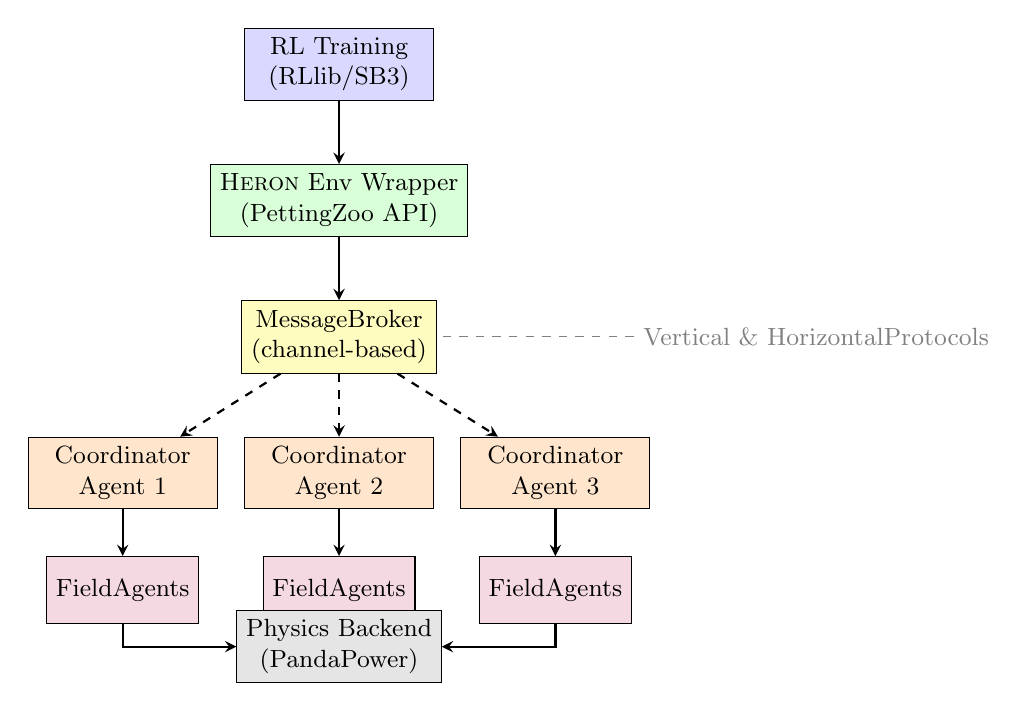
\begin{tikzpicture}[
    node distance=0.8cm,
    box/.style={rectangle, draw, minimum width=2.4cm, minimum height=0.85cm, align=center, font=\small},
    arrow/.style={->, >=stealth, thick},
    dasharrow/.style={->, >=stealth, thick, dashed}
]
% RL Layer
\node[box, fill=blue!15] (rl) {RL Training\\(RLlib/SB3)};

% Environment Layer
\node[box, fill=green!15, below=of rl] (env) {\heron{} Env Wrapper\\(PettingZoo API)};

% Message Broker
\node[box, fill=yellow!25, below=of env] (broker) {MessageBroker\\(channel-based)};

% Coordinator Agents
\node[box, fill=orange!20, below left=0.8cm and 0.3cm of broker] (ca1) {Coordinator\\Agent 1};
\node[box, fill=orange!20, below=0.8cm of broker] (ca2) {Coordinator\\Agent 2};
\node[box, fill=orange!20, below right=0.8cm and 0.3cm of broker] (ca3) {Coordinator\\Agent 3};

% Field Agents
\node[box, fill=purple!15, below=0.6cm of ca1, minimum width=1.9cm] (f1) {FieldAgents};
\node[box, fill=purple!15, below=0.6cm of ca2, minimum width=1.9cm] (f2) {FieldAgents};
\node[box, fill=purple!15, below=0.6cm of ca3, minimum width=1.9cm] (f3) {FieldAgents};

% Physics
\node[box, fill=gray!20, below=3.0cm of broker] (physics) {Physics Backend\\(PandaPower)};

% Arrows
\draw[arrow] (rl) -- (env);
\draw[arrow] (env) -- (broker);
\draw[dasharrow] (broker) -- (ca1);
\draw[dasharrow] (broker) -- (ca2);
\draw[dasharrow] (broker) -- (ca3);
\draw[arrow] (ca1) -- (f1);
\draw[arrow] (ca2) -- (f2);
\draw[arrow] (ca3) -- (f3);
\draw[arrow] (f1.south) |- (physics.west);
\draw[arrow] (f3.south) |- (physics.east);

% Protocol annotation
\node[right=2.5cm of broker, font=\small, text=gray] (proto) {Vertical \& Horizontal\\Protocols};
\draw[gray, dashed] (proto) -- (broker);

\end{tikzpicture}
\caption{\heron{} architecture (power-system case study). A MessageBroker mediates agent communication via named channels. CoordinatorAgents manage FieldAgents through vertical protocols. The environment owns horizontal protocols for peer coordination.}
\label{fig:architecture}
\end{figure}

%------------------------------------------------------------------------------
\subsection{Hierarchical Agent Architecture}
\label{sec:hierarchy}
%------------------------------------------------------------------------------

Many CPS are naturally hierarchical: fast local controllers, mid-level coordinators, and supervisory operators. \heron{} formalizes this with a three-level agent hierarchy:

\begin{itemize}[nosep]
    \item \textbf{Level 1 (FieldAgent)}: Local sensing and actuation with \texttt{owner+public} visibility. Examples: individual devices, sensors, actuators.
    \item \textbf{Level 2 (CoordinatorAgent)}: Manages subordinate FieldAgents with \texttt{upper\_level+owner+public} visibility. Examples: zone controllers, aggregators.
    \item \textbf{Level 3 (SystemAgent)}: Global coordination with \texttt{system} visibility. Examples: central operators, market coordinators.
\end{itemize}

\paragraph{Dual execution modes.}
\heron{} supports two execution patterns:

\begin{enumerate}[nosep]
    \item \textbf{Synchronous mode}: Direct \texttt{observe()} $\rightarrow$ \texttt{act()} calls within \texttt{env.step()}. Simple, fast, suitable for centralized training (CTDE).
    \item \textbf{Event-driven mode}: Discrete-event simulation via \texttt{EventScheduler} with configurable timing. Agents \texttt{tick()} independently at heterogeneous rates with realistic delays.
\end{enumerate}

This dual-mode design enables training in synchronous mode (fast iteration, shared rewards) and validation in event-driven mode (realistic distributed execution with latencies).

\paragraph{Event-driven execution via discrete-event simulation.}
The event-driven mode (Algorithm~\ref{alg:event-driven}) uses a priority-queue \texttt{EventScheduler} where each agent has a \texttt{tick()} method:
\begin{itemize}[nosep]
    \item Agents \textbf{tick independently} at configurable intervals (\texttt{tick\_interval})
    \item \textbf{Configurable delays}: observation delay (\texttt{obs\_delay}), action effect delay (\texttt{act\_delay}), message delivery delay (\texttt{msg\_delay})
    \item \textbf{Optional jitter}: Uniform or Gaussian randomization via \texttt{TickConfig} for robustness testing
    \item Supports \textbf{heterogeneous decision rates} across the agent hierarchy
\end{itemize}

\begin{algorithm}[t]
\caption{Event-driven execution via \texttt{EventScheduler}}
\label{alg:event-driven}
\begin{algorithmic}[1]
\REQUIRE EventScheduler with priority queue, registered agents with TickConfig
\STATE \textbf{def} run\_until(t\_end):
\STATE \hspace{0.5cm} \textbf{while} queue not empty \textbf{and} current\_time $<$ t\_end:
\STATE \hspace{1.0cm} event $\gets$ pop\_min(queue) \COMMENT{Get earliest event}
\STATE \hspace{1.0cm} current\_time $\gets$ event.timestamp
\STATE
\STATE \hspace{1.0cm} \textbf{if} event.type == AGENT\_TICK:
\STATE \hspace{1.5cm} agent $\gets$ agents[event.agent\_id]
\STATE \hspace{1.5cm} obs $\gets$ agent.observe(state\_at(t - obs\_delay)) \COMMENT{Delayed observation}
\STATE \hspace{1.5cm} action $\gets$ agent.act(obs)
\STATE \hspace{1.5cm} schedule(ACTION\_EFFECT, t + act\_delay, action) \COMMENT{Delayed action}
\STATE \hspace{1.5cm} schedule(AGENT\_TICK, t + tick\_interval) \COMMENT{Next tick}
\STATE
\STATE \hspace{1.0cm} \textbf{else if} event.type == ACTION\_EFFECT:
\STATE \hspace{1.5cm} apply\_action(event.agent\_id, event.payload)
\STATE
\STATE \hspace{1.0cm} \textbf{else if} event.type == MESSAGE\_DELIVERY:
\STATE \hspace{1.5cm} broker.deliver(event.payload) \COMMENT{Delayed message}
\end{algorithmic}
\end{algorithm}

%------------------------------------------------------------------------------
\subsection{Composable Observability with FeatureProviders}
\label{sec:observability}
%------------------------------------------------------------------------------

Observations are assembled from composable \textbf{FeatureProviders}. Each provider maps a slice of state into a vector and declares visibility scopes.

\begin{table}[t]
\centering
\caption{Visibility scopes in \heron{}.}
\label{tab:visibility}
\small
\begin{tabular}{@{}lp{3.3cm}p{6.6cm}@{}}
\toprule
\textbf{Scope} & \textbf{Who can access} & \textbf{Example signals} \\
\midrule
\texttt{public} & All agents & System time, global alerts, market prices \\
\texttt{owner} & Owning agent only & Device SOC, internal costs, local setpoints \\
\texttt{upper\_level} & Parent in hierarchy & Subordinate aggregates, boundary conditions \\
\texttt{system} & System-level (L3) agents & Full network state, all bus voltages/line flows \\
\bottomrule
\end{tabular}
\end{table}

\paragraph{Visibility logic.}
The \texttt{is\_observable\_by()} method implements access control:
\begin{itemize}[nosep]
    \item \texttt{public}: All agents observe.
    \item \texttt{owner}: Only the owning agent (requestor\_id == owner\_id).
    \item \texttt{upper\_level}: Agents one level above the owner.
    \item \texttt{system}: System-level agents (level $\geq$ 3).
\end{itemize}

This enables \textbf{systematic observability ablations}: benchmarks can progressively restrict visibility (\eg \texttt{system} $\rightarrow$ \texttt{upper\_level} $\rightarrow$ \texttt{owner}) to quantify information requirements.

%------------------------------------------------------------------------------
\subsection{MessageBroker for Explicit Communication}
\label{sec:messaging}
%------------------------------------------------------------------------------

\heron{} decouples agent communication from observation through a \textbf{MessageBroker} abstraction.

\paragraph{Key abstractions.}
\begin{itemize}[nosep]
    \item \textbf{Channels}: Named communication paths with standardized naming convention: \texttt{env\_\{id\}\_\_action\_\_\{parent\}\_to\_\{child\}}.
    \item \textbf{Publish/Consume}: Agents publish messages to channels; recipients consume asynchronously.
    \item \textbf{Environment isolation}: Channel names include environment ID for multi-environment training.
\end{itemize}

\paragraph{Implementation.}
The default \texttt{InMemoryBroker} is thread-safe and suitable for single-process training. The interface supports extension to distributed backends (Kafka, RabbitMQ) for deployment.

%------------------------------------------------------------------------------
\subsection{Protocol System for Coordination}
\label{sec:protocols}
%------------------------------------------------------------------------------

\heron{} separates \emph{coordination semantics} from \emph{physics} through a modular protocol system.

\paragraph{Protocol composition.}
Each protocol combines:
\begin{enumerate}[nosep]
    \item \textbf{CommunicationProtocol}: What messages are exchanged (prices, bids, setpoints).
    \item \textbf{ActionProtocol}: How received messages translate to actions.
\end{enumerate}

\paragraph{Vertical protocols (hierarchical).}
Owned by CoordinatorAgents for top-down control:
\begin{itemize}[nosep]
    \item \textbf{SetpointProtocol}: Centralized---coordinator directly assigns subordinate actions.
    \item \textbf{PriceSignalProtocol}: Decentralized---coordinator sends price signals; subordinates optimize locally.
\end{itemize}

\paragraph{Horizontal protocols (peer-to-peer).}
Owned by the environment for cross-hierarchy coordination:
\begin{itemize}[nosep]
    \item \textbf{P2PTradingProtocol}: Market clearing for resource exchange between peers.
    \item \textbf{ConsensusProtocol}: Distributed averaging via gossip (extensible interface).
\end{itemize}

This design enables controlled comparisons: under identical observability, compare centralized dispatch vs. price-based coordination vs. peer trading.

%==============================================================================
\section{Power Systems Case Study}
\label{sec:power}
%==============================================================================

We instantiate \heron{} for multi-microgrid coordination using PandaPower AC power flow. The goal is to demonstrate a concrete CPS benchmark where information structure and coordination protocols matter.

\paragraph{Provided assets.}
\begin{itemize}[nosep]
    \item \textbf{Standard networks}: IEEE 13/34/123-bus and CIGRE LV feeders via PandaPower.
    \item \textbf{Device models}: Generators, energy storage systems (ESS), tap-changing transformers.
    \item \textbf{FeatureProviders}: 14 domain-specific providers (Table~\ref{tab:features}).
    \item \textbf{Protocols}: Setpoint, price signal (vertical); P2P trading (horizontal).
    \item \textbf{Examples}: Single microgrid, multi-microgrid P2P, MAPPO training, distributed execution.
\end{itemize}

\begin{table}[t]
\centering
\caption{FeatureProviders in the power systems case study.}
\label{tab:features}
\small
\begin{tabular}{@{}llp{5.8cm}@{}}
\toprule
\textbf{FeatureProvider} & \textbf{Typical Visibility} & \textbf{Description} \\
\midrule
ElectricalBasePh & owner, upper\_level & Active/reactive power (P, Q), voltage (V) \\
PowerLimits & owner & Min/max generation capacity \\
StorageBlock & owner, upper\_level & SOC, capacity, charge/discharge limits, degradation \\
StatusBlock & public & Device availability, on/off state \\
TapChangerPh & owner & Transformer tap position and limits \\
InverterBasedSource & owner & Inverter mode, reactive capability \\
BusVoltages & system, upper\_level* & Voltage magnitudes/angles (*boundary buses) \\
LineFlows & system & Branch flows, loading percentages \\
NetworkMetrics & public, system & Total generation, load, losses \\
ThermalLoading & owner, upper\_level & Line thermal limits and loading \\
PhaseConnection & owner & Bus connection, phase information \\
StepState & public & Timestep, episode progress \\
VoltVarCurve & owner & Volt-VAR control curves \\
ShuntCapacitorBlock & owner & Capacitor bank state \\
\bottomrule
\end{tabular}
\end{table}

\paragraph{Agent mapping.}
\begin{itemize}[nosep]
    \item \textbf{DeviceAgent} (FieldAgent): Controls individual DERs (generator, ESS, transformer).
    \item \textbf{GridAgent} (CoordinatorAgent): Manages a microgrid's devices, integrates power flow.
\end{itemize}

\paragraph{Benchmark questions enabled.}
\begin{itemize}[nosep]
    \item \textbf{Minimum observability}: What visibility scope is sufficient for stable operation?
    \item \textbf{Privacy-preserving coordination}: Can microgrids coordinate without revealing internal SOC/costs?
    \item \textbf{Protocol sensitivity}: Which protocol is more robust under constrained information?
    \item \textbf{Centralized-to-distributed mismatch}: Do policies trained with full observability fail under realistic filtering?
\end{itemize}

%==============================================================================
\section{Experiments}
\label{sec:experiments}
%==============================================================================

We present pilot experiments demonstrating \heron{}'s benchmark capabilities. Values marked with $\dagger$ are preliminary; full baseline sweeps will accompany the public release.

\subsection{Observability Ablation}

Using FeatureProviders, we train MAPPO agents under progressively restricted visibility.

\begin{table}[h]
\centering
\caption{Observability ablation (IEEE 34-bus, 3 microgrids, summer peak scenario).}
\label{tab:observability-ablation}
\small
\begin{tabular}{@{}lccccc@{}}
\toprule
\textbf{Observability} & \textbf{Cost (\$)} & \textbf{Degradation} & \textbf{Safety Viol. (\%)} & \textbf{Converge (ep)} \\
\midrule
System (full) & \exampleval{859} & Baseline & \exampleval{2.1} & \exampleval{2400} \\
Upper-level & \exampleval{891} & \exampleval{+3.7\%} & \exampleval{2.8} & \exampleval{2600} \\
Owner-only & \exampleval{1024} & \exampleval{+19\%} & \exampleval{8.7} & \exampleval{4200} \\
Public-only & \exampleval{1543} & \exampleval{+80\%} & \exampleval{24} & Fails \\
\bottomrule
\end{tabular}
\end{table}

\textbf{Finding}: Upper-level visibility provides a favorable trade-off---modest cost increase (+3.7\%) while respecting privacy boundaries. Public-only visibility fails to converge, highlighting minimum information requirements.

\subsection{Centralized-to-Distributed Mismatch}

We train with full visibility (direct mode) and evaluate under upper-level visibility (distributed mode).

\begin{table}[h]
\centering
\caption{Train/test visibility mismatch.}
\label{tab:mismatch}
\small
\begin{tabular}{@{}lccc@{}}
\toprule
\textbf{Train Visibility} & \textbf{Test Visibility} & \textbf{Cost (\$)} & \textbf{Degradation} \\
\midrule
System & System & \exampleval{859} & -- \\
Upper-level & Upper-level & \exampleval{891} & +3.7\% \\
\midrule
\textbf{System} & \textbf{Upper-level} & \exampleval{1055} & \textbf{+23\%} \\
\bottomrule
\end{tabular}
\end{table}

\textbf{Finding}: Policies trained with system-level access degrade significantly (-23\%) when deployed with realistic information constraints. This motivates training under target observability.

\subsection{Protocol Comparison}

Under identical upper-level observability, we compare coordination protocols.

\begin{table}[h]
\centering
\caption{Protocol comparison (upper-level visibility, 3 microgrids).}
\label{tab:protocol}
\small
\begin{tabular}{@{}lccc@{}}
\toprule
\textbf{Protocol} & \textbf{Cost (\$)} & \textbf{Coordination Overhead} & \textbf{Privacy} \\
\midrule
Setpoint (centralized) & \exampleval{891} & Low & None \\
Price Signal & \exampleval{912} & Medium & Partial \\
P2P Trading & \exampleval{928} & High & Full \\
\bottomrule
\end{tabular}
\end{table}

\textbf{Finding}: Centralized setpoint achieves lowest cost but requires full control authority. P2P trading preserves privacy at modest cost premium (+4\%).

%==============================================================================
\section{Cross-Domain Applicability}
\label{sec:generalization}
%==============================================================================

While this paper presents a power systems case study, \heron{}'s abstractions are domain-agnostic. The framework applies to systems with:
\begin{itemize}[nosep]
    \item \textbf{Hierarchical organization}: Local $\rightarrow$ regional $\rightarrow$ central control.
    \item \textbf{Information partitioning}: Role-based visibility, privacy constraints.
    \item \textbf{Explicit coordination}: Protocols beyond implicit state sharing.
\end{itemize}

Examples include traffic networks (signals $\rightarrow$ intersections $\rightarrow$ districts), robot fleets (robots $\rightarrow$ zone managers $\rightarrow$ warehouse control), and supply chains (facilities $\rightarrow$ regions $\rightarrow$ network).

The power case study serves as a reference template: users extend \texttt{FieldAgent}, implement domain-specific \texttt{FeatureProviders}, and configure protocols for their application.

%==============================================================================
\section{Limitations and Future Work}
\label{sec:limitations}
%==============================================================================

\textbf{Current limitations.}
\begin{itemize}[nosep]
    \item \textbf{Communication realism}: We support channel-based messaging with configurable delays and jitter, but do not yet model packet loss or bandwidth constraints.
    \item \textbf{Dynamic observability}: Visibility rules are configuration-driven; learning or negotiating information access is future work.
    \item \textbf{Latency distributions}: Current jitter supports uniform and Gaussian distributions; domain-specific profiles (SCADA-like, V2X-like) are future work.
\end{itemize}

\textbf{Power domain limitations.}
\begin{itemize}[nosep]
    \item \textbf{Balanced network assumption}: The PandaPower backend targets balanced operation; unbalanced three-phase models require extension.
    \item \textbf{Solver robustness}: Power flow non-convergence handling is not yet benchmarked.
\end{itemize}

\textbf{Roadmap.}
\begin{itemize}[nosep]
    \item Domain-specific latency profiles (SCADA-like, V2X-like) for timing studies.
    \item Distributed MessageBroker backends (Kafka, RabbitMQ) for deployment validation.
    \item Additional domain instantiations (traffic, robotics) to validate cross-domain reuse.
    \item Standardized observability/protocol leaderboards.
\end{itemize}

%==============================================================================
\section{Conclusion}
\label{sec:conclusion}
%==============================================================================

We presented \heron{}, a hierarchical multi-agent framework built around a single organizing principle: \textbf{multi-agent simulation should make execution model, information structure, and coordination mechanisms explicit}. \heron{} provides:
\begin{itemize}[nosep]
    \item A three-level agent hierarchy with dual execution modes: synchronous for training and event-driven (via \texttt{EventScheduler} with configurable delays and jitter) for realistic validation.
    \item FeatureProviders with visibility labels for systematic observability control.
    \item A MessageBroker abstraction for explicit, channel-based communication.
    \item Composable vertical and horizontal protocols for coordination studies.
\end{itemize}

We demonstrated benchmark readiness through a power systems case study with standard networks, 14 FeatureProviders, and reference protocols. Pilot experiments show that observability constraints significantly impact learning and that train/test visibility mismatch causes substantial performance degradation---findings that highlight the importance of treating information structure as a benchmark variable.

\heron{} is released open-source to support reproducible research on information-constrained multi-agent coordination. By providing configurable observability and protocols as experimental controls, \heron{} enables systematic studies of how information constraints affect MARL in cyber-physical systems.

%==============================================================================
% References
%==============================================================================

\bibliographystyle{plainnat}
\bibliography{references}

%==============================================================================
% Appendix
%==============================================================================
\newpage
\appendix

\section{Hyperparameters}
\label{app:hyperparams}

\begin{table}[h]
\centering
\caption{MAPPO training hyperparameters.}
\small
\begin{tabular}{@{}ll@{}}
\toprule
\textbf{Parameter} & \textbf{Value} \\
\midrule
Learning rate & $3 \times 10^{-4}$ \\
Discount factor ($\gamma$) & 0.99 \\
GAE lambda ($\lambda$) & 0.95 \\
Clip parameter ($\epsilon$) & 0.2 \\
Entropy coefficient & 0.01 \\
Value loss coefficient & 0.5 \\
Max gradient norm & 0.5 \\
Batch size & 4096 \\
Minibatch size & 256 \\
PPO epochs & 10 \\
Number of workers & 4 \\
Network architecture & [256, 256] MLP \\
Activation & ReLU \\
\bottomrule
\end{tabular}
\end{table}

\section{Network Specifications}
\label{app:networks}

\begin{table}[h]
\centering
\caption{Test network specifications (power case study).}
\small
\begin{tabular}{@{}lcccc@{}}
\toprule
\textbf{Network} & \textbf{Buses} & \textbf{Lines} & \textbf{Voltage (kV)} & \textbf{Peak Load (MW)} \\
\midrule
IEEE 13-Bus & 13 & 11 & 4.16 & 3.5 \\
IEEE 34-Bus & 34 & 33 & 24.9 & 1.77 \\
IEEE 123-Bus & 123 & 127 & 4.16 & 3.49 \\
CIGRE LV & 14 & 13 & 0.4 & 0.245 \\
\bottomrule
\end{tabular}
\end{table}

\section{Safety Metric Definitions}
\label{app:safety}

\begin{align}
V_{\text{voltage}} &= \sum_{b \in \mathcal{B}} \left[\max(0, V_b - 1.05) + \max(0, 0.95 - V_b)\right] \\
V_{\text{loading}} &= \sum_{l \in \mathcal{L}} \max(0, \text{Loading}_l - 1.0) \\
V_{\text{SOC}} &= \sum_{s \in \mathcal{S}} \left[\max(0, 0.1 - \text{SOC}_s) + \max(0, \text{SOC}_s - 0.9)\right]
\end{align}

Voltage limits: 0.95--1.05 p.u. Line loading limit: 100\%. SOC safe range: 10--90\%.

\section{Code Availability}
\label{app:code}

\heron{} is available at: \url{https://github.com/Criss-Wang/PowerGym}

Installation:
\begin{verbatim}
pip install -e ".[all]"  # Full installation
pip install -e ".[powergrid]"  # Power grid case study only
\end{verbatim}

\end{document}w